\section{The Particle Flow Algorithm}

\begin{figure}
	\centering
	\begin{subfigure}{1\textwidth}
		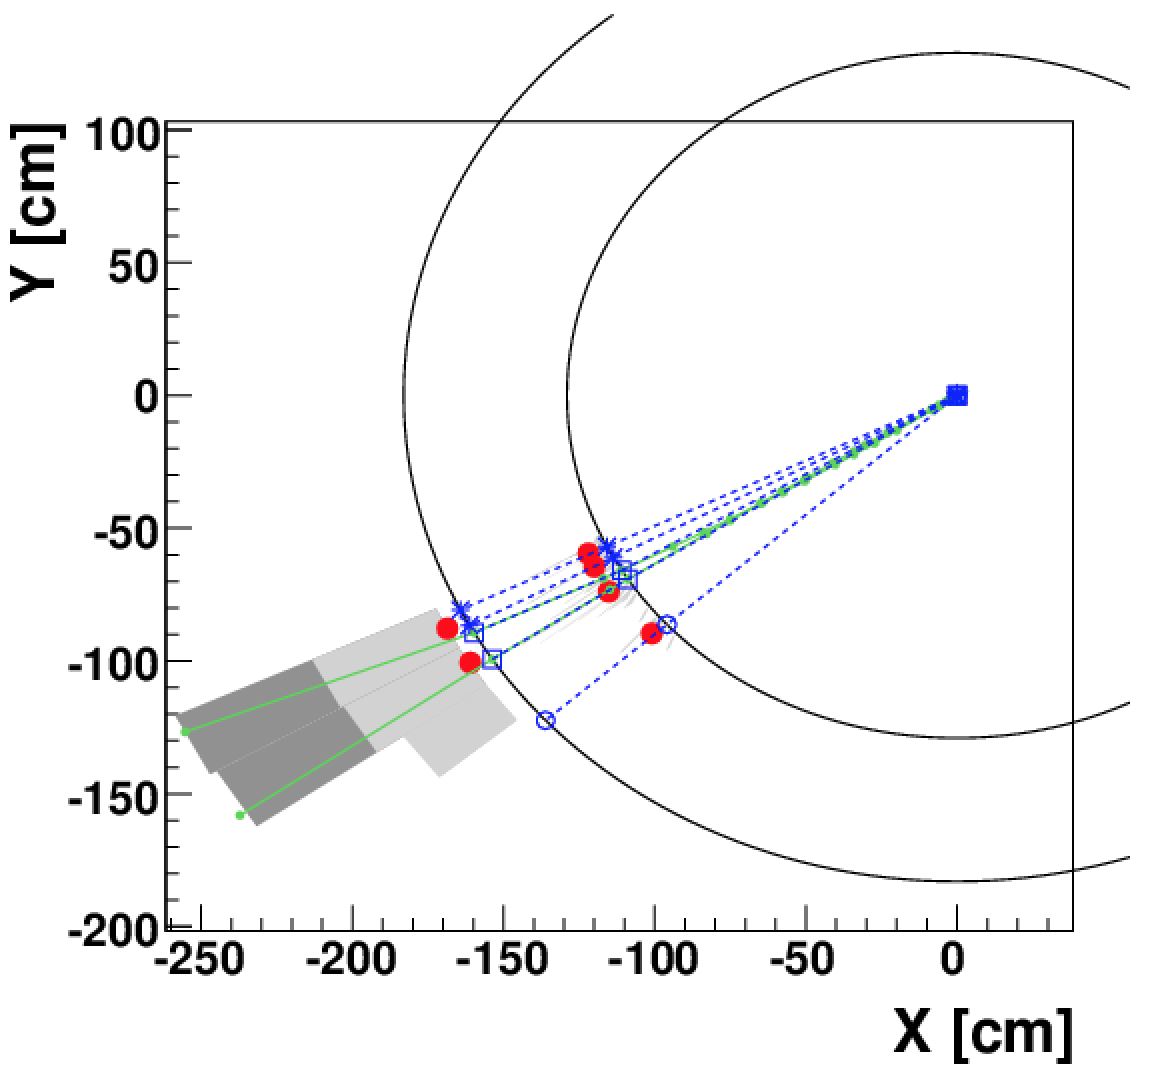
\includegraphics[width=.8\linewidth]{analysis/pics/PF_a.png}
		\caption{The $(x, y)$ view.}
		\label{fig:PF_a}
	\end{subfigure}
	
	\begin{subfigure}{.4\textwidth}
		\centering
		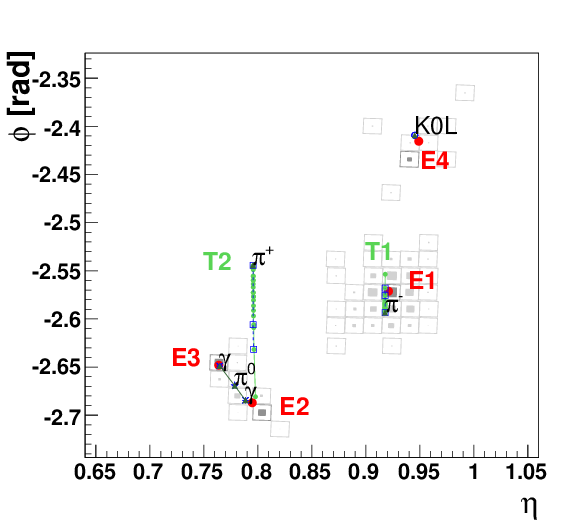
\includegraphics[width=.8\linewidth]{analysis/pics/PF_b.png}
		\caption{The $(\eta,\phi)$ view on ECAL.}
		\label{fig:PF_b}
	\end{subfigure}
		\begin{subfigure}{.4\textwidth}
			\centering
			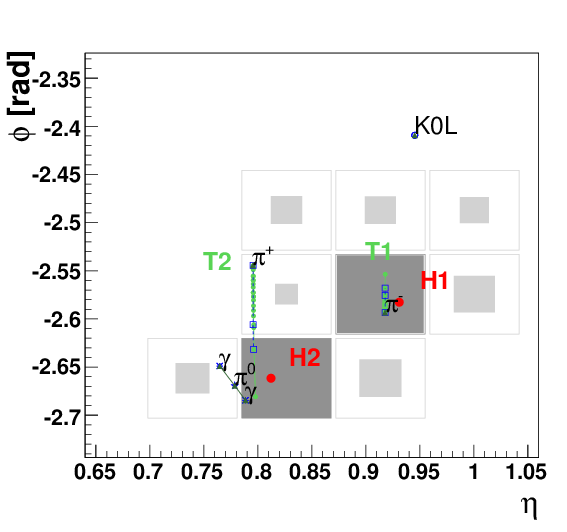
\includegraphics[width=.8\linewidth]{analysis/pics/PF_c.png}
			\caption{The $(\eta,\phi)$ view on HCAL.}
			\label{fig:PF_c}
		\end{subfigure}%
	\caption{An event display of a simple hadronic jet in the $(x, y)$ view (Figure \ref{fig:PF_a}) and in the $(\eta,\phi)$ view, where $\eta$ stands for pseudo-rapidity and $\phi$ for the azimuthal angle, on the ECAL surface (Figure \ref{fig:PF_b}) and the HCAL surface (Figure \ref{fig:PF_c}). (These two surfaces are represented as two circles centred around the interaction point in the first view.) The $K^{0}_{L}$, the $\pi^{-}$ and the two photons from the $\pi^{0}$ decay are detected as four well separated ECAL clusters (Figure \ref{fig:PF_b}). The $\pi^{+}$ leaves no energy in the ECAL. The two charged pions are reconstructed as charged-particle tracks, appearing as vertical solid lines in the $(\eta,\phi)$ views and circular arcs in the $(x, y)$ view. These tracks point towards two HCAL clusters (Figure \ref{fig:PF_c}). In all three views, the cluster positions are represented by dots, the simulated particles by dashed lines, and the position of their impact on the calorimeter surfaces by various open markers.}
	\label{fig:PF_event_display}
\end{figure}

\clearpage

\section {The Tau Lepton reconstruction}

With a lifetime of $2.9\times10^{−13}$ s and a mass of 1776.82 \mev the $\tau$ is the heaviest of the leptons. It was discovered between 1974 and 1977 by the team under Martin Perl while studying the $e^{+}+e^{-}\longrightarrow e^{\pm}+\mu^{\mp}$. The $\tau$ decays leptonically, with a branching ratio of $17\%$ for each channel, via the following decay $\tau\longrightarrow\nu_{\tau}W^{*}\longrightarrow\nu_{\tau}l\nu_{l}$. However the most important decay channel is the hadron one with a total branching fraction of $\sim 65\%$. Among all the possible hadronic decays as shown on Table \ref{table:tau_hdecay} the ones called "one-prong", where only one charged hadron is produced, are the most frequent.

\begin{figure}[tbh!]
	\begin{center}	
			\begin{tabular}{ | c | c | c | c |}
				\hline
				Decay Mode & Resonance & Mass [\mev] & BF (\%) \\ \hline
				\hline
				$\tau^{-}\longrightarrow h^{-}\nu_{\tau}$& $\pi$ & 139.6 & 11.6 \\ \hline
				$\tau^{-}\longrightarrow h^{-}\pi^{0}\nu_{\tau}$& $\rho$ & 770 & 26.0 \\ \hline
%				$\tau^{-}\longrightarrow h^{-}\pi^{0}\pi^{0}\nu_{\tau}$ & $a_{1}$ & 1200 & \\ 10.8 \hline
				$\tau^{-}\longrightarrow h^{-} h^{+} h^{-} \nu_{\tau}$& $a_{1}$& 1200 & 9.8 \\ \hline
				$\tau^{-}\longrightarrow h^{-} h^{+} h^{-} \pi^{0}\nu_{\tau}$& & & 4.8 \\ \hline
				other hadronic channels& & & 1.7 \\ \hline
				\hline
				total & & & 64.8 \\ \hline
				\hline
			\end{tabular}
		\caption{ Hadronic tau decay modes into either one or three charged hadrons h and potential $\pi_{0}$, and the corresponding branching fractions BF. Also shown are the intermediate resonances and their masses, which are used in some of the tau reconstruction algorithms.}
		\label{table:tau_hdecay}
	\end{center}
\end{figure}

\clearpage
\section {The Jet reconstruction}

